\documentclass[a4paper,11pt]{article}

\usepackage[utf8]{inputenc}
\usepackage[T1]{fontenc}
\usepackage[french]{babel}
\usepackage{amsmath, amsthm, amssymb}
\usepackage[left=2cm, right=2cm, top=2cm, bottom=2cm]{geometry}
\usepackage[lined,boxed]{algorithm2e}
\usepackage{graphicx}

\title{Rapport : Angry Birds}
\author{François \sc{Pirot} \and Grégoire \sc{Beaudoire}}
\date{\today}

\begin{document}

\maketitle

\tableofcontents

\section*{Introduction}
\addcontentsline{toc}{section}{Introduction}

Dans le cadre du module Projet 1, nous avons travaillé en binôme sur 
un projet de programmation en ocaml. Le but était de réaliser en premier
lieu un simulateur de billard, avant de l'adapter en un jeu se rapprochant
du célèbre jeu Angry Birds pour mobile.

Ce projet, d'une durée de 6 semaines, exploite une grande partie des fonctionnalités
graphiques proposées par ocaml. Il s'agit de créer deux simulateurs - un billard,
et un jeu que l'on nommera Angry Balls - les plus fonctionnels possibles pour
l'utilisateur. Celui-ci pourra alors profiter d'une interface utilisateur entièrement
implémentée dans la fenêtre graphique d'ocaml.

En premier lieu, nous nous intéresserons à notre billard, son fonctionnement, 
et les enjeux majeurs rencontrés lors de son implémentation. 
Ensuite, nous verronscomment nous l'avons adapté en notre jeu Angry Balls, et nous 
pencherons notamment sur les difficultés auxquelles nous avons dû faire face pour ce faire.
Enfin, nous reviendrons sur les interfaces utilisateur des deux simulateurs, sensiblement
similaires, qui les rendent vraiment fonctionnels.

\section {Le billard}
Commençons donc avec notre billard. La première chose à considérer est la manière dont on
va le représenter en ocaml.

\subsection{Les structures de données}
Plusieurs éléments vont intervenir dans notre billard. Il s'agit de les définir tous, et d'en
optimiser l'utilisation avec des fonctions de manipulation adéquates.

\subsubsection{Les vecteurs}
L'entité de base à considérer est le vecteur. Nous le rencontrons inévitablement dans
un projet nécessitant un moteur physique, et nous en faisant plusieurs utilisations différentes.
L'implémentation des vecteurs doit donc être suffisamment générique pour que nous puissions
les utiliser confortablement dans n'importe quel contexte. 

Techniquement, son implémentation est très simple : le type vecteur est un type enregistrement
renseignant ses coordonnées cartésiennes dans le plan. Un vecteur $v$ aura alors pour coordonnées 
$(v.x,v.y)$.

Nous avons alors besoin de fonctions de manipulation de base sur ces vecteurs : l'addition, la soustraction,
le produit scalaire, la multiplication par un scalaire, et la norme.

\subsubsection{Les boules}
Nous pouvons maintenant nous intéresser au premier élément concret dans notre billard : la boule.
Cette dernière peut être caractérisée par une très grande quantité de caractéristiques ; il a fallu
choisir lesquelles conserver absolument, et desquelles nous pouvions nous passer.

Ainsi, une boule $b$ est repérée par trois vecteurs : sa position $b.o$, sa vitesse $b.v$, et son accélération $b.a$. 
Est également renseigné son rayon. Nous avons décidé de ne pas implémenter de masse à nos boules,
ce qui aurait été très difficile à implémenter sur le plan moteur physique, pour une amélioration
moindre étant donné que les boules d'un billard sont sensiblement de la même masse.

Ce type boule est très pratique car il resert pour beaucoup d'autres objets utiles dans notre billard.

\subsubsection{Les trous}
Les trous de notre billard sont en fait considérés comme des boules particulières, puisqu'elles sont
inconsistantes, à savoir qu'il n'y a pas de collision entre un trou et une vraie boule, et fixes. 
Leur vitesse et accélération sont donc fixées au vecteur nul, et restent inchangées.

\subsubsection{Le billard}
Le billard est délimité par les bords de la fenêtre graphique, à l'exception du bord haut où est affichée
la barre utilisateur, qui affiche le score des joueurs et contient les boutons pour relancer la partie
ou pour fermer le billard.

Il contient par défaut 6 trous, placés selon les conventions d'un billard conventionnel, et autant
de boules que souhaité, dans la limite du possible. Pour faciliter la manipulation directe des boules
(et aussi des trous), ces dernières sont répertoriées dans un tableau et non dans une liste. Cela
implique qu'une boule supprimée pendant la partie n'est pas vraiment supprimée du billard. Elle reste
dans le tableau des boules, mais est placée en fin de tableau, tandis que l'information du nombre de
boules réelles dans le billard est décrémentée. 

Enfin, le billard contient l'information du coefficient de frottement $f \leqslant 1$ que subissent 
les boules qui s'y déplacent. A chaque nouveau pas de calcul, on multiplie la vitesse de chaque boule
par ce coefficent de frottement.

\subsection{Le moteur physique}
Maintenant que la structure de billard est implémentée, il s'agit de gérer les mouvements des boules
à l'intérieur de ce dernier. Cela implique tous les rebonds contre les bords du billard, entre deux
ou trois boules, ou encore l'intéraction des trous sur les boules.

\subsubsection{Le déplacement élémentaire}
On gère le déplacement des boules par intervalles de temps réguliers, et suffisamment courts pour que
l'on puisse gérer le mouvement par la méthode d'Euler au premier ordre. On fixe alors l'intervalle de
temps séparant deux frames à $dt := 0.01s$. Cette valeur a été choisie de telle sorte qu'une boule
ne puisse pas se déplacer d'une distance supérieure à son rayon pendant $dt$. Ainsi, avec des boules
de rayon $20 pixels$, nous pouvons autoriser des vitesses allant jusqu'à $2000 pixels/s$ dans le 
billard. Ces vitesses seront bornées par la méthode de lancement des boules, sur laquelle nous reviendrons
dans la suite.

Ainsi, en utilisant la méthode d'Euler, nous obtenons donc les formules suivantes :
\[b.o(t + dt) = b.o(t)\times f + b.v(t)\times dt\]
\[b.v(t + dt) = b.v(t)\times f + b.a(t)\times dt\]

Dans des conditions de base, l'accélération des boules est toujours nulle.

\subsubsection{L'intéraction entre une boule et un bord du billard}
Lorsqu'une boule commence à sortir du billard, ou en l'occurence de la fenêtre graphique, il faut
corriger son déplacement pour gérer le rebond de la boule contre le bord du billard correspondant.

Nous introduisons un type direction : \texttt{type direction = Haut | Bas | Droite | Gauche | Nil}, qui va
nous permettre de déterminer sur quel bord la boule doit rebondir, la valeur \texttt{Nil} correspondant à
une boule qui ne sort pas du billard.

Ainsi, dès qu'une boule déborde de la fenêtre graphique, on commence par la replacer de sorte qu'elle
touche juste le bord dans lequel elle est rentrée, puis on fait une symétrie verticale de son vecteur
vitesse dans les cas \texttt{Droite} ou \texttt{Gauche}, et horizontale dans les cas \texttt{Haut} ou \texttt{Bas}.

Il est important de bien replacer la boule juste contre le bord, sinon elle risque de toujours déborder
de la fenêtre graphique au pas de calcul suivant, malgré la correction du déplacement, à cause de l'atténuation
des vitesses. Il en résulte que la boule est emprisonnée contre le bord, duquel elle ne parvient pas à
se dégager, ce qui n'est bien sûr pas souhaitable.

\subsubsection{L'intéraction entre deux boules}
Lorsque deux boules s'intersectent, c'est qu'elles se sont rentrées dedans. Là encore, il va falloir
corriger leurs trajectoire pour prendre leur collision en compte.

Il faut tout d'abord séparer les deux boules $b1$ et $b2$, de sorte qu'elles ne se chevauchent plus, mais qu'elles
soient presque en contact. On supprime le contact de cette manière, afin d'éviter le problème décrit
avec le rebond contre le bord du billard : on ne veut pas que les boules restent collées entre elles
sans pouvoir se séparer. On effectue cette séparation en conservant une sorte de barycentre $g$ entre les
deux boules, chacune pondérée par le rayon de l'autre :
\[g := \frac{b2.r \times b1.o + b1.r \times b2.o}{b1.r + b2.r} \]
\\On replace ensuite les boules à partir de ce barycentre $g$ selon leur vecteur directeur, d'une distance
égale à leur rayon multiplié par $1.01$ (afin d'assurer le quasi-contact entre les deux boules).

On peut calculer le vecteur de déviation généré par la collision des deux boules $b1$ et $b2$. On commence
par calculer un vecteur directeur unitaire $\vec{u_{12}}$ entre les deux boules, dirigé selon la droite
reliant leurs deux centres. Le vecteur de déviation $\vec{dv}$ s'obtient alors par la formule suivante :
\[\vec{dv} := (\vec{v1} . \vec{u_{12}} - \vec{v2} . \vec{u_{12}}) \ \vec{u_{12}}. \]
\\Puis on obtient les nouvelles vitesses par les formules suivantes :
\[\vec{v1} \leftarrow \vec{v1} - \vec{dv}\]
\[\vec{v2} \leftarrow \vec{v2} + \vec{dv}\]

\subsubsection{L'intéraction entre trois boules}
Pour améliorer la gestion des collisions au sein de notre billard, et notamment lorsque la concentration
des boules est importante, nous traitons le cas particulier où trois boules entrent en collision simultanément.
Cela intervient notamment au tout début de la partie, lorsque les boules sont organisées en un triangle qui
maximise les contacts entre les boules qui le composent.

On réutilise pour ce cas la gestin du contact entre deux boules. On considère que lors de la collision d'une
boule avec deux autres simultanément, l'énergie du choc est équitablement répartie entre les deux boules.
Ainsi, la collision triple entre les boules b1, b2 et b3 se résumera à 3 collisions doubles - entre les boules
b1 et b2, b2 et b3, et b1 et b3 - où les vitesses considérées sont toutes divisées par deux.

\subsubsection{L'intéraction entre une boule et un trou}
La condition d'intéraction entre une boule et un trou est un peu différente de celle entre deux boules :
il ne suffit plus que les deux se chevauche, il faut maintenant que la distance entre le centre de la boule
et celui du trou soit inférieure au rayon du trou.
\begin{figure}[h]
\caption{Intéraction Boule/Trou}
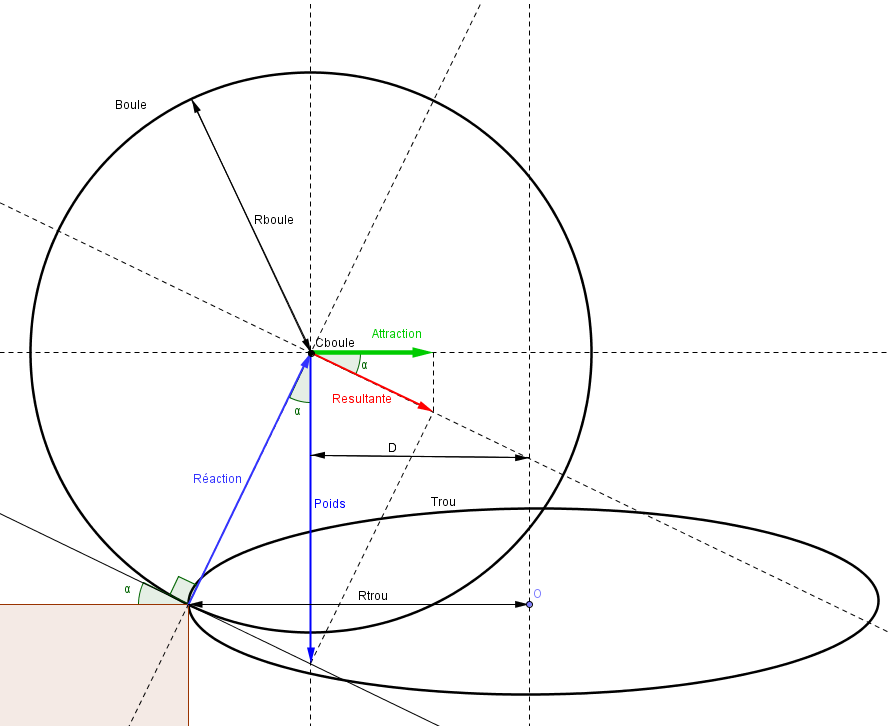
\includegraphics[scale = 0.7]{schema.png}
\end{figure}

Dans ce cas de figure, un calcul pas trop compliqué permet de déduire la valeur de l'attraction du trou
sur la boule en fonction de la distance $D$ entre les centres du trou et de la boule.
\begin{eqnarray}
&d& := \frac{Rtrou - D}{Rboule} \nonumber \\
&\alpha& = \arcsin d \nonumber \\
&Resultante& = Poids \sin \alpha \nonumber \\
&Attraction& = Resultante \cos \alpha = Poids \sin \alpha \cos \alpha = Poids \times d \sqrt{1 - d^2} \nonumber
\end{eqnarray}
Il ne nous reste donc plus qu'à choisir une valeur arbitraire pour $Poids$. Cette valeur doit être
suffisamment élevée pour qu'une boule avec une grande vitesse tombe tout de même dans le trou quand elle
passe par dessus. La valeur choisie dans notre programme est donc fixée à $100000$. Cette valeur de l'attraction
est alors tout simplement entrée dans l'accélération de la boule lorsque celle-ci rentre en intéraction avec un
trou. C'est le seul cas où l'accélération d'une boule peut être non nulle dans notre billard.

Bien sûr, la condition de suppression d'une boule qui rencontre un trou est qu'elle soit entièrement contenue
dans ce trou, à savoir que $ D \leqslant Rtrou - Rboule $.

\subsection{Utilisation d'un quadtree pour améliorer le simulateur}

\subsubsection{La structure quadtree}

\subsubsection{Construction d'un quadtree}

\subsubsection{Utilisation du quadtree}

\subsection{Lancement d'une partie de billard}
Nous avons désormais tous les outils nécessaires pour commencer à pouvoir vraiment jouer avec notre simulateur
de billard. Il faudra choisir les règles à imposer dans notre billard, et la façon d'intéragir avec celui-ci.

\subsubsection{Lancement d'un coup de billard}
Lorsque c'est au tour d'un joueur de jouer, celui-ci va tirer dans une boule, puis le billard évolue jusqu'à
ce que toutes les boules s'imobilisent. 

On différencie alors une boule des autres : la boule blanche, qui est la seule que l'on est autorisé à lancer.
Ainsi, au début de chaque tour, l'utilisateur doit sélectionner cette boule qu'il désire lancer, puis cliquer
dans la direction dans laquelle il veut tirer, aussi loin de sa position de départ qu'il souhaite tirer fort.
Si le premier clic a été effectué en $(x1,y1)$ et le second en $(x2,y2)$, alors en donne à la boule lancée le
vecteur vitesse $\vec{v} = K(x2-x1,y2-y1)$, où $K$ est une constante choisie de telle sorte que les vitesses
soient convenablement bornées au sein de notre billard. Nous avons choisi la valeur $K=5$.

On fait ensuite tourner notre simulateur, frame par frame. A chaque tour de boucle, on fait évoluer les boules
sans prendre en compte le collisions, puis on teste pour tous les couples de boules si elles se sont rentrées
dedans, auquel cas on teste si une troisième boule est en contact avec ces deux autres. On gère si c'est le cas
la collision triple, ou double. On effectue un test sur tous les couples (trou,boule) pour gérer les intéractions
quand elles ont lieu d'être. Enfin, on gère le rebond de chacune des boules sur les bords du billard quand elles
commencent à sortir de la fenêtre graphique.

On arrête le tour lorsque les vitesses des boules sont toutes
inférieures à une certaine valeur fixée comme une approximation de vitesse nulle. Dans notre billard, cette
vitesse seuil vaut $vmin = 30 pixels/s$. Alors le tour change, et il faut à nouveau tirer dans la boule blanche.

Il y a une autre condition d'arrêt possible : dans le cas où la boule blanche tombe dans un trou au cours du
tour. Alors le tour s'arrête, et l'utilisateur va devoir replacer cette boule blanche à un endroit correct,
puis la relancer pour un nouveau tour. Les vitesses des autres boules sont conservées pendant la phase de 
replacement, ce qui fait que le billard se relance comme il s'était interrompu au tour suivant.

La suppression d'une boule se fait en échangeant sa position avec la dernière dans le sous-tableau contenant
les boules encore présentes dans le billard, puis en décrémentant le nombre \texttt{n} de boules dans le billard.
La boule blanche est la boule d'indice $0$ dans le tableau. Avant chaque tour, on en effectue une copie, si bien
que quand elle est détruite, on réinsère cette copie dans le tableau, qui est ensuite replacée convenablement
par l'utilisateur.

\subsubsection{L'organisation d'une partie}
Une partie de billard se joue entre deux joueurs concurrents. Les tours s'alternent au cours de la partie, au
cours desquels les joueurs marquent des points en rentrant le plus de boules possible dans les trous, et la
partie s'arrête quand il ne reste plus que la boule blanche sur le plateau. Est alors déclaré vainqueur le 
joueur ayant marqué le plus de points.

Le billard est initialisé avec 36 boules rouges à rentrer dans les trous, disposées en un triangle de 8 rangées,
et la boule blanche leur faisant face de l'autre côté du billard. Les diamètres des boules rouges valent $20 pixels$, 
celui de la boule blanche en fait $16$, et ceux des trous en font $32$.

Le système de comptage de point valorise le joueur qui parvient à rentrer un grand nombre de boules en un tour.
Ainsi, il marquera $100 \times i$ points pour la i-ème boule rentrée au cours de son tour, sauf si cette boule
est la boule blanche, auquel cas son tour s'arrête.

\section{Angry Balls}
Nous avons désormais à notre disposition un simulateur de billard complet, avec un moteur physique fonctionnel.
Il s'agit maintenant de l'adapter pour obtenir notre jeu Angry Balls.

\subsection{Les modifications dans la structure de données}
Nous réutilisons la structure de donnée du billard en rajoutant et supprimant quelques éléments.

\subsubsection{Les boules}
Désormais, les boules vont pouvoir être détruites au cours de la partie. Il faut donc leur rajouter un champ, 
à savoir la solidité. Chaque boule aura donc une solidité définie par un flottant positif au début de la partie,
et cette valeur va diminuer à chaque choc suffisamment violent entre la boule et un élément du niveau. Une
boule sera détruite lorsque sa solidité deviendra négative. Là encore on caractérise une boule spéciale, la boule
projectile, qui ne peut être détruite, qui a pour solidité initiale le flottant \texttt{infinity}.

\subsubsection{Les obstacles}
Pour pimenter un peu les niveaux, nous rajoutons un nouveau type d'objet, à savoir les obstacles. Ce sont en
fait des murs plantés dans le sol, indestructibles, et ayant comme extrémité supérieure un bord arrondi, représenté
par une boule fixe et de solidité infinie. 

\subsubsection{Le type niveau}
Le type niveau est le type billard auquel on a supprimé les trous, que l'on a remplacés par des obstacles.
Les boules de billard sont évidemment remplacées par les boules avec solidité. Enfin, le niveau n'a comme bord
que celui du bas, représentant le sol. Ainsi, une boule est également supprimée lorsqu'elle sort du niveau, par
la gauche ou par la droite (et non par le haut, car la gravité peut la faire retomber dans le niveau).

\subsection{Un moteur physique plus évolué}
Bien que l'on réutilise en grande partie les notions physiques introduites pour le moteur physique du billard,
la jeu Angry Balls en fait intervenir des nouvelles qui apportent leur lot de difficultés.

\subsubsection{L'ajout de la gravité}
La grande nouveauté dans le jeu Angry Balls par rapport au billard est le fait que les boules sont désormais
plongées dans un champs de gravitation constant $\vec{g}$ orienté vers le sol, et de norme arbitraire.

Cela n'ajoute pas grand chose aux fonction calculant l'évolution élémentaires des boules dans le niveau :
\[b.o(t + dt) = b.o(t)\times f + b.v(t)\times dt\]
\[b.v(t + dt) = b.v(t)\times f + b.a(t)\times dt\]
\[b.a(t + dt) = (0,g) \texttt{ sauf contre-indication}\]

\subsubsection{La réaction du support}
Nous rencontrons alors une première difficulté : si une boule est posée sur le sol, elle subit la réaction de
ce sol, qui compense son poids. Ainsi, l'accélération à laquelle elle est soumise devient nulle. Cette condition
est cependant facilement vérifiable par un test sur l'altitude à laquelle se trouve le centre de la boule : si elle
est au niveau de la valeur du rayon de la boule (ou très légèrement au-dessus), nous lui imposons une accélération
nulle. 

Les choses se compliquent quelque peu lorsque ce n'est plus le sol le support, mais une autre boule $b1$ sur laquelle
s'appuie la boule $b2$ que nous considérons. Nous considérons alors dans une approche simplifiée que la boule support
se comporte comme une boule fixe, et que la réaction qui en découle est celle d'un support fixe de forme circulaire.
La compensation de l'accélération de la boule $b2$ est alors la suivante : 
\[ \vec{a_2} \leftarrow \vec{g} - (\vec{g} . \vec{u_{12}}) \ \vec{u_{12}} \]
Si le contact persiste, c'est donc effectivement que la boule $b1$ constitue un support pour la boule $b2$, et notre
approche est justifiée. Si le contact ne persiste pas, alors l'accélération de la boule $b2$ est réinitialisé à $\vec{g}$
dès la frame suivante, et les répercutions de notre manipulation sont quasi-inexistantes. Notre gestion de la réaction
d'une boule sur une autre est donc bien justifiée.

\subsubsection{Collision avec le sol}
La collision avec le sol se gère de la même manière que la collision avec le bord bas dans un billard. Il faut
cependant rajouter la fragilisation de la boule ayant rebondi sur le sol. Cette fragilisation $ds$ est proportionnelle
à la déviation du vecteur vitesse de la boule, qui vaut le double de sa composante verticale :
\[ ds := K \times 2 \times b.v.y \texttt{ où K est une constante arbitraire, 4 dans nos fonctions.}\]

\subsubsection{Collision entre deux boules}
En ce qui concerne la collision entre deux boules, elle reste inchangée dans le cas traditionnel. On doit alors
fragiliser les deux boules, de manière proportionnelle au vecteur de déviation résultant de la collision :
\[ ds := K \times \| \vec{dv} \| \texttt{ où K est la constante choisie dans la formule précédente.}\]

En revanche, dans le cas où une boule $b$ est détruite au cours de la collision, la déviation $\vec{dv'}$ résultante est d'autant
moins importante que l'énergie nécessaire à la destruction de la boule était faible :
\[ \vec{dv'} := \frac{b.s}{ds} \ \vec{dv} \]

\subsubsection{Collision avec un obstacle}
La collision avec un obstacle se gère de la même manière qu'avec le sol lorsque la boule rebondit sur la partie
murée de l'obstacle. Lorsqu'elle rencontre la partie arrondie de l'obstacle, la collision se comporte comme une
collision entre deux boules, à la différence que la deuxième boule étant ici fixe, le vecteur déviation $\vec{dv}$
est donc multiplié par deux, et ne s'applique qu'à la boule rencontrant l'obstacle. Evidemment, cette multiplication
par deux se reporte également sur la fragilisation $ds$ de la boule.

\subsection{Déroulement d'une partie}
Nous avons finalement réussi à détourner toutes les nouvelles difficultés rencontrées lors de l'implémentation
du comportement des éléments qui composent notre niveau d'Angry Balls. Nous pouvons maintenant passer à l'implémentation
d'une partie dans notre jeu.

\subsubsection{Lancement d'un tour}
Au début de son tour, l'utilisateur va devoir lancer la boule projectile, exactement de la même manière
que dans le billard. Cela donne une vitesse à cette dernière, et la simulation du niveau peut alors
commencer. 

Lorsque les boules atteignent une vitesse inférieure au seuil, cela ne veut plus forcément dire que l'évolution
du niveau est figée : en effet, ce n'est pas parce qu'une boule est quasi-immobile qu'elle va le rester, à
cause de la gravitation. Pour éviter d'arrêter le tour alors que le niveau est instable et peut encore évoluer,
on laisse à l'utilisateur le soin de choisir quand il souhaite passer au tour suivant. Ce choix ne lui est proposé
qu'une fois que les vitesses des boules sont passées sous le seuil souhaité, auquel cas il n'a qu'à effectuer
un clic de souris pour passer au tour suivant. Alors la boule projectile est replacée dans la zone de lancement,
et attend d'être relancée.

Le score se compte de la même manière que dans le billard : 100 * i points pour la i-ème boule détruite pendant le
tour.

\subsubsection{Gagner un niveau}
Deux niveaux ont été implémentés dans notre jeu Angry Balls, mais rien n'empêche à l'utilisateur d'en implémenter
d'autres s'il s'en sent le courage et l'envie. Un menu de choix de niveau apparaît à l'ouverture du jeu, et à 
chaque reset. L'utilisateur clique sur le numéro du niveau qu'il souhaite tenter, et celui-ci se lance.

Pour réussir le niveau, le joueur a le droit à trois lancers pour détruire ou sortir du niveau toutes les boules
rouges ennemies. Son score est compté au fur et à mesure que les boules sont détruites, et s'il réussit le niveau,
son score s'affiche dans une fenêtre de fin de niveau qui lui propose de rejouer. S'il ne réussit pas le niveau au
bout de ses trois lancers autorisés, la même fenêtre s'affiche, lui indiquant qu'il a perdu, et lui proposant de 
réessayer.

\end{document}
